% !TEX root = ../Rulebook.tex

In the medium term, the \RCAW aims to transfer specific aspects of industrial scenarios in the tests and to demonstrate the practical applicability of the solutions. The challenges, which are adapted or redefined annually, serve as a test platform for the further development of the competitions. Each technical challenge is separately awarded. That means, teams can participate in any number of them. Hoewever any challenge will only be awarded if at least two teams competed unless the only competing team provided an outstanding performance.

A challenge increases the level capabilities of a robot in \RCAW related to:

\begin{itemize}
  \item \textbf{Variability of the environmental conditions} ... The setup conditions of a run are designed variably including disturbances. The lighting situations in the arena are changed dynamically, the configuration of the tables (height, format) is adapted or manipulation objects are mixed with unknown decoy objects.
  \item \textbf{Complexity of the scenarios} ... New arena elements are involved in a scenario
  or its dimensions (size, duration) are increased. This includes, for example, multi-robot scenarios, assembly tasks or new interaction stations.
\end{itemize}

For a successful implementation either an existing solution has to be increased in robustness or a new approach for an additional task has to be developed. The challenges here lie in the fields of perception, manipulation, navigation and planning.

\begin{figure}[h!]
  \centering
  \begin{tikzpicture}
  	\begin{polaraxis}[
        xtick ={0, 90, 180, 270},
        xticklabels= {Manipulation, Perception, Navigation, Planning},
        width=5.5cm,
        height=5.5cm,
        legend pos=outer north east,
    ]
  	\addplot
  		coordinates {(0,1.5) (90,3) (180, 0.5) (270,0.5) (0, 1.5)};  % cp
      \addlegendentry{Cluttered Pick Test}
    \addplot
    	coordinates {(0,3) (90,1.5) (180,1) (270,1) (0,3)};  % pfd
      \addlegendentry{Pick from Drawer Test}
  	\end{polaraxis}
  \end{tikzpicture}
  \label{Examplary Challenge introducing a long term operation based on an extended Final test}
\end{figure}

The challenges of 2021 focussing on perception and manipuation in two scenarios. While "Cluttered Pick Test" (CP) adresses the robustness of perception, the "Pick from Drawer Test" (PFD) is focused on additional complexity by including objects in a drawer. Additonally, the start of a league specific simulator, to ease entry of new teams and enable better scientific evaluation is to be established through Simulation Evaluation Test (SE).


\newpage
\section{Cluttered Pick Test}

\subsection{Purpose and Focus of the Test}
The purpose of the \iaterm{Cluttered Pick Test}{CPT} is to evaluate the perception
and manipulation of the robots in a cluttered scenario. The scenario is motivated by
the fact that most of the objects in the factory or labs are always lying in a clutter.


\subsection{Scenario Environment}
The arena used for this test contains basically all elements as for the Basic
Manipulation Test. Two service areas with a height of 10cm are involved in the test,
most probably near to each other. The objects mentioned by the referee box will be placed
on both the service areas.(see Fig.~\ref{fig:clutter})  
All geometrical definitions given in Fig.~\ref{fig:manipulation_zone} are considered here \textbf{except 
for the rule of min 0.02m distance between objects} . The objects here can be placed near to each other,
or on top of each other. 

\begin{figure} [h!]
\begin{center}
\subfloat[]{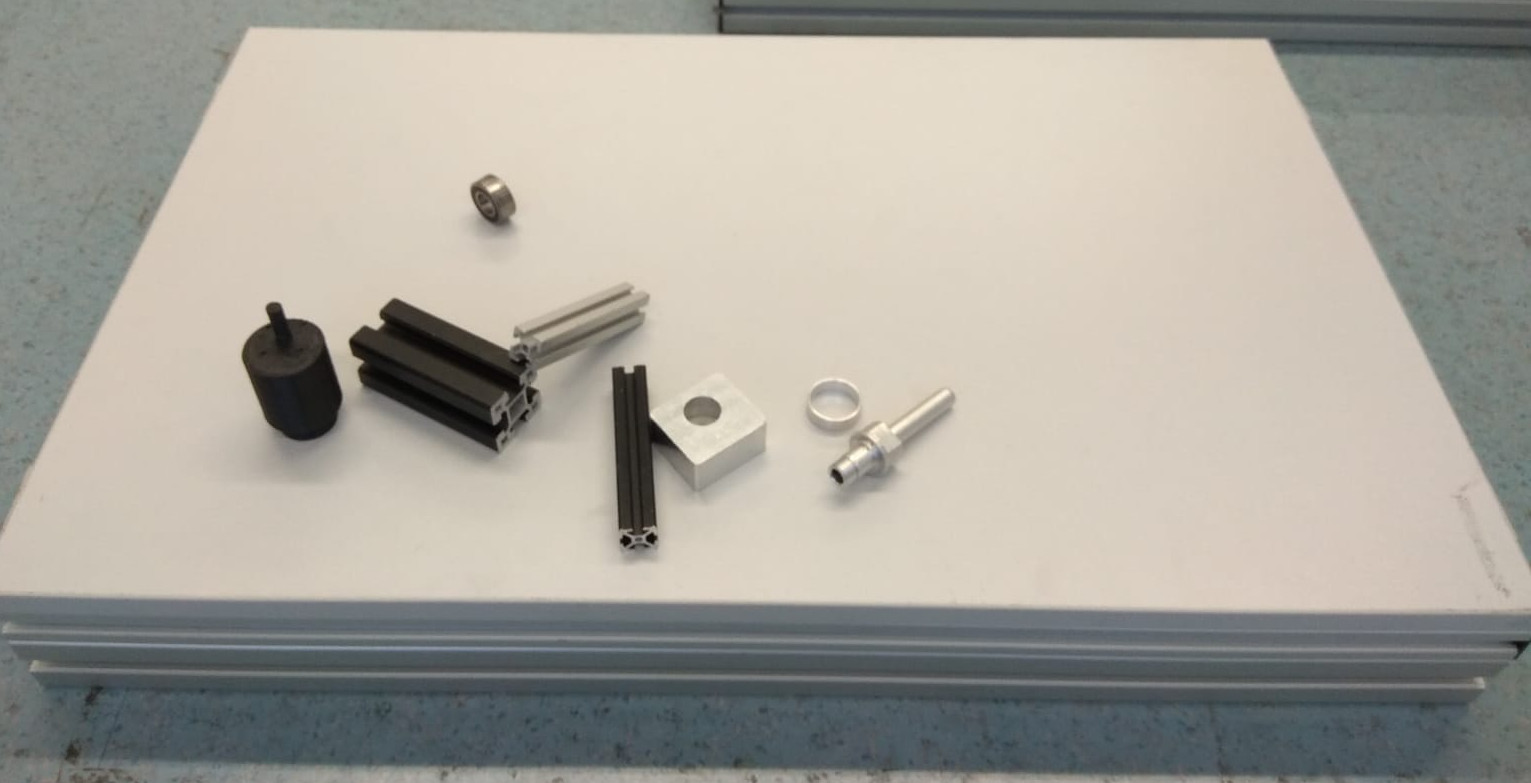
\includegraphics[height = 3cm]{./images/cluttered_pick_1.jpg}} \hspace{1cm}
\subfloat[]{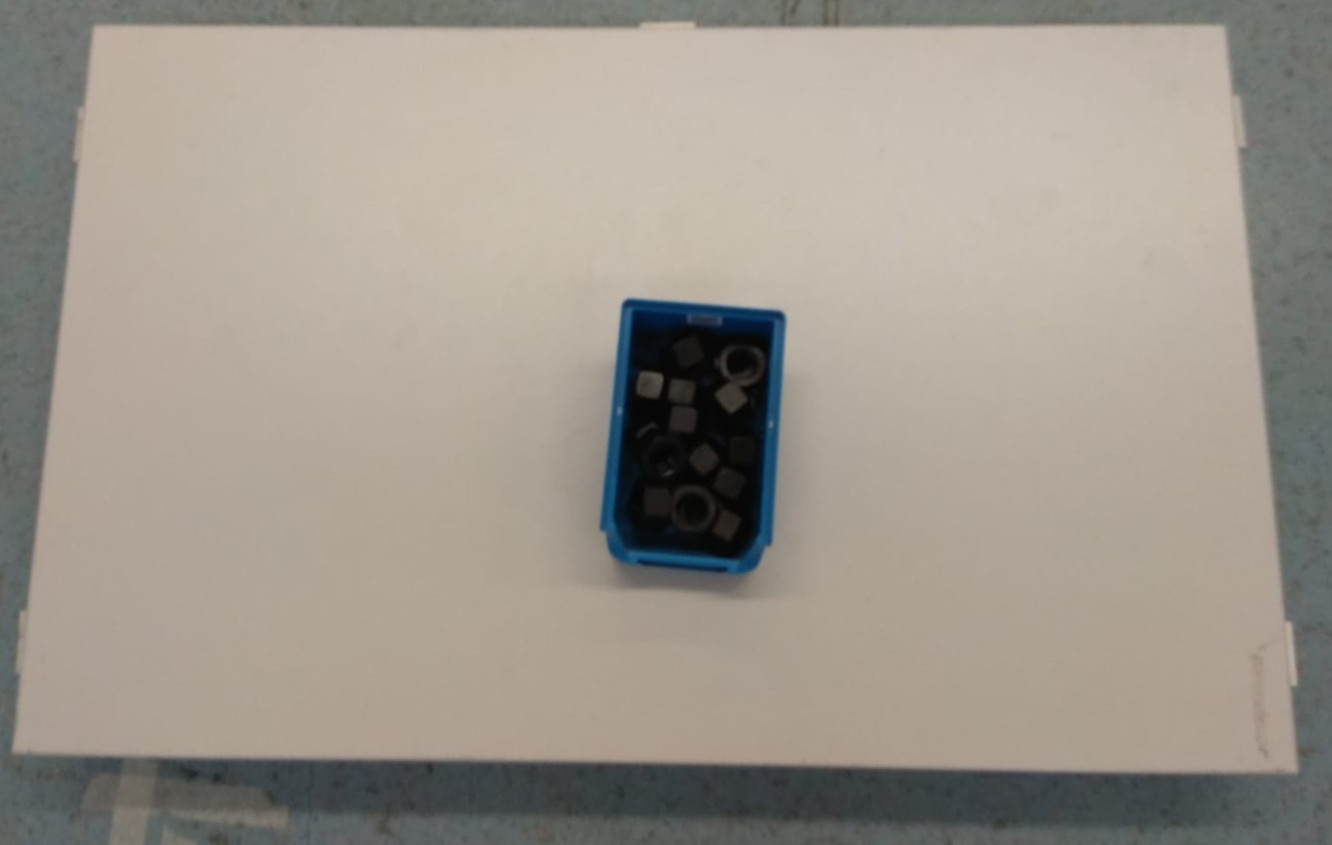
\includegraphics[height = 3cm]{./images/cluttered_pick_2.jpg}}
\end{center}
\caption{objects places in cluttered environment}
\label{fig:clutter}
\end{figure}


\subsection{Variation}
A slight variation in the competition will be to run with 2 robots simultaneously competing with each other.
For fairness of the competition the organizers should ensure that the distance between the robot starting 
point and the corresponding service station be equal.
 
\subsection{Task}
The robot starts at the defined start position outside the arena.
The task consists of navigating to the specified service area containing all the 
requested object. The robot localizes and identifies the object and picks.
The task consists of a sequence of grasp operations. The objective is to pick up all 3 instance of the requested type and avoid picking other objects.
\par
The task specification consists of:
\begin{itemize}
	\item[--] The specification of the initial place
	\item[--] A source location, given as place (e.g. \texttt{WS09})
	\item[--] A list of objects to be manipulated from the source location.
	\item[--] The specification of a final place for the robot
\end{itemize}

\paragraph{Manipulation Objects}
The manipulation objects used in this test are defined by the instances described in Table~\ref{tab:Instances}.

\subsection{Rules}
The following rules have to be obeyed:

\begin{itemize}
\item A single robot is used.
\item The robot has to start from outside the arena and to end in the final.
\item The order in which the teams have to perform will be determined by a draw.
\item At the beginning of a team's period, the team will get the task specification.
\item A service area counts as successfully reached as defined in Section~\ref{ssec:Navigating}
\item Three objects have to be picked.
\item There will be 3-5 decoy objects that must not be picked on the service area.
\item A manipulation object counts as successfully grasped as specified in Section~\ref{ssec:GraspingObjects}.
\item The run is over when the robot reached the final place or the designated time has expired.
\end{itemize}

\subsection{Scoring}
\begin{itemize}
\item 100 points are awarded for each correctly and successfully picked object
\item -50 points for every incorrectly picked object
\item 25 points for reaching the correct service area
\item 25 points for reaching the final position
\end{itemize}

\newpage
\section{Pick from Drawer Test}

\szug{Should we think about additional rules for collisions?}

\szug{I think an individual drawer avoids unpredictable configurations but generates of course additional effort. Probably we think about a "standard drawer construction" for 2021?}

\szug{Should we include one or two decoy objects that are placed by a referee to avoid scripted solutions.}

\subsection{Purpose and Focus of the Test}
The collection of freely available objects lying on a manipulation zone is the core capability of \RCAW-robots. The \iaterm{Pick from Drawer Test}{PFD} goes beyond this level and considers objects stored in drawers too. In this way, the challenge
extends the idea of the shelf where the robot has to plan the grasping operation in a limited space but it is not necessary to interact with the environment.

\subsection{Scenario Environment}
The first version of the challenge gives much freedom to the teams. They can choose an arbitrary drawer configuration. The drawer is wholly covered in the beginning and can only be linearly moved in one direction. The surrounding construction has to remain at its position.

\par
Robot's movements must open the drawer directly. Self-driven, automatic solutions integrated into the drawer system are not allowed.
The rules do not define the handling mechanism itself, the teams are completely free to design an appropriate concept. Any handle, knob, hole, or connector mounted to the drawer is permitted. Based on this interaction, the drawer has to be moved at least \textcolor{red}{15 cm}.

\subsection{Task}
The drawer setup is located at an arbitrary position. The drawer contains at least one but not more than three  manipulation objects described in Table~\ref{tab:Instances}. It is stored directly on bottom of the drawer. Any other content is not permitted!

The team configures the objects and the drawer during preparation phase.

\textcolor{red}{This test does not adress navigation capabilities. Hence the robot can start the run everywhere.} It moves directly to the drawer, open it, grasps the objects and place them in robot`s repository.

\subsection{Rules}
The following rules have to be obeyed:

\begin{itemize}
\item A single robot is used.
\item The test runs for 5 minutes.
\item \textcolor{red}{The robot can start at an arbitrary position inside or outside the arena.}
\item The order in which the teams have to perform will be determined by a draw.
\item Each team is responsible for preparing the drawer system. The team selects the objects and places them within the drawer.
\item The drawer is opened by at least \textcolor{red}{15cm}.
\item A manipulation object counts as successfully grasped as specified in Section~\ref{ssec:GraspingObjects}. \textcolor{red}{It is not necessary to place the objects at another manipulation zone.}
\item The run is over when the designated time has expired.
\end{itemize}

\subsection{Scoring}
\begin{itemize}
\item 100 points for opening the drawer
\item 100 points are awarded for each correctly and successfully picked object
\item Time bonus of one point per second after collecting 3 objects successfully.
\end{itemize}

\newpage
\section{Simulation Evaluation Test}

\subsection{Purpose and Focus of the Test}

The purpose of this test is to provide the RoboCup @Work League with new capabilities. These capabilities are the option to do scientific evaluation regarding stochastic behaviour and scalability analysis. This provide the competing teams with the option of using their experimental results in scientific papers and provide a stronger link to the scientific robotic communities.

Another aspect is the option to add integration tests and continuous integration to the workflow of the teams to provide better management of software versions. Additionally, this provides the team members with the capabilities to learn state-of-the-art software development techniques.

Finally, a simulation adds the option for new teams to start with a virtual robot excluding the typical hardware problems associated with real robots. This eases the entry into the league and paves the way for a larger growth of the league in regard to participating teams in the future. 

\subsection{Scenario Environment}

The scenario for this test is to enable teams using a (partial) simulation to show these to the league. Finally, the league may be able to choose a default simulation environment to provide support for this environment in the future. 

Consequently, the simulation of the team competing in this challenge needs to fulfill some requirements:

\begin{description}
  \item[Free to be used:] The simulation software needs to be usable by competing teams free of charge. The software does not need to be open source.
  \item[Open-Source API:] The interface of the simulation needs to be open source. Especially, the implementation of the robot specific functions and behaviours, like executing movement commandos and outputting laser scanner data etc.\ needs to be implemented in a way that allows for easy modification of interested teams.
  \item[Official Models:] The simulated arena environment need to contain the 3D-Model of the official repository of the @Work League \url{https://github.com/robocup-at-work/models}. Additionally, the tasks to be executed need to be generated by the official Referee Box, see Section~\ref{sec:refbox}
\end{description}

  Within the simulation environment one of the tasks specified in Section~\ref{sec:tests} needs to be executed.

\subsection{Task}

The task of this challenge is to show the execution of one of the tasks defined in Section~\ref{sec:tests} in the virtual environment. However, this task is not graded regarding the normal scoring scheme. The evaluation of this task is based on the behaviour of the simulation itself. Relevant aspects that are considered in the scoring are the precision and speed of the simulation. To this end, the teams shall provide stochastic data on the precision of multiple runs of their simulation  as well as the speed of the simulation expressed as a real-time-factor (Quotient between time passed in the simulation and time passed in the real world). Additionally, the teams need to indicate the API of their simulation as well as the used simulation software and its license. The task execution may either be shown in a video or live. 

\subsection{Rules}

\begin{itemize}
  \item Virtual representation based on the object and table definitions from \url{https://github.com/robocup-at-work/models}
  \item Virtual representation of the teams robot
  \item Free to use (for robotic teams) simulation software / environment
  \item Execution of a task as specified in Section~\ref{sec:tests}
  \item Start of task by Referee Box see Section~\ref{sec:refbox}
  \item Task execution as video or live
  \item Indication of precision in form of reproduction accuracy (execute multiple times and compare results)
  \item Indication of simulation speed based on real-time factor (Quotient between virtual clock speed and real world time)
\end{itemize}

\subsection{Scoring}

Referees grade task execution and simulation based on the following criteria:
\begin{itemize}
  \item Up to 100 Points for Ease of Use
  \item Up to 100 Points for Visualization
  \item Up to 200 Points for Precision
  \item Up to 200 Points for Speed
  \item Up to 300 Points for Simulation Capabilities
\end{itemize}



\newpage
\section{New Objects Transportation Test}

\subsection{Purpose and Focus of the Test}
The collection of freely available objects lying on a manipulation zone is the core capability of \RCAW-robots. The \iaterm{New Objects Transportation Test }{NOT} includes a new and realistic objects set to grasp. The challenge extends the standard Basic Transportation Test~\ref{sec:Basic Transportation Test} where the robot has transport only basic objects.

\subsection{Scenario Environment}
Basically the BTT2 scenario will be used but with the objects defined in section~\ref{sec:new_objects}. This includes all basic manipulation objects from Table \ref{manipulation_objects} and future objects from Table~\ref{tab:new_objects1} and Table~\ref{tab:new_objects2}.

\subsection{Task}
The task is the same as for a BTT2, with the modification that rocking objects will be replaced by the objects from section~\ref{sec:new_objects}. 


\subsection{Rules}
The following rules have to be obeyed:

\begin{itemize}
	\item A single robot is used.
	\item Six objects have to be picked.
	\item There must be at least 3 decoy objects which must not be picked.
	\item The robot has to start from outside the arena and to stop in the goal area.
	\item A manipulation object counts as successfully grasped as specified in Section~\ref{ssec:GraspingObjects}.
	\item The run is over when the robot reached the final place and the human worker successfully assembled the components or the designated time has expired.
	\item The order in which the teams have to perform will be determined by a draw.
	\item At the beginning of a team's period, the team will get the task specification.
\end{itemize}

\subsection{Scoring}
\begin{itemize}
	\item 200 points are awarded for each correctly and successfully picked object
	\item 125 points are awarded for each correctly placed object.
	\item Standard scoring applies for all other aspects
\end{itemize}

\newpage
\section{Robot-Human Interaction Test}

\subsection{Purpose and Focus of the Test}
The collection of freely available objects lying on a manipulation zone is the core capability of \RCAW-robots. The \iaterm{Robot Human Interaction Test }{RHI} includes not only a new and realistic objects set to grasp but also includes human workers into the scenario. In this way, the challenge extends the standard Basic Transportation Test~\ref{sec:Basic Transportation Test} where the robot has transport only basic objects without any further interaction. 

\subsection{Scenario Environment}
Basically the BTT2 scenario will be used but with the objects defined in section~\ref{sec:new_objects}. This includes all basic manipulation objects from Table \ref{manipulation_objects} and future objects from Table~\ref{tab:new_objects1} and Table~\ref{tab:new_objects2}.

\subsection{Task}
The task is the same as for a BTT2, with the modification that rocking objects will be replaced by the objects from section~\ref{sec:new_objects}. Furthermore a human worker has to be selected which has to assemble suitable parts together. The human worker has to stand outside the arena and has to be able to collect items from goal workspaces. Additional tools, screws, nuts and washers needed can be carried and prepared by the human worker.
Objects which can be assemble: 
\begin{itemize}
	\item Screw M20\_100 and Spacer and Nut M20
	\item Bearing2 and  Housing
	\item Axis2 and Nut M20  
\end{itemize}

\subsection{Rules}
The following rules have to be obeyed:

\begin{itemize}
	\item A single robot is used.
	\item Six objects have to be picked.
	\item There must be at least 3 decoy objects which must not be picked.
	\item The robot has to start from outside the arena and to stop in the goal area.
	\item A manipulation object counts as successfully grasped as specified in Section~\ref{ssec:GraspingObjects}.
	\item The run is over when the robot reached the final place and the human worker successfully assembled the components or the designated time has expired.
	\item The order in which the teams have to perform will be determined by a draw.
	\item At the beginning of a team's period, the team will get the task specification.
\end{itemize}

\subsection{Scoring}
\begin{itemize}
	\item 200 points are awarded for each correctly and successfully picked object
	\item 125 points are awarded for each correctly placed object.
	\item 50 points are awarded for successfully assembled components.
	\item Standard scoring applies for all other aspects
\end{itemize}

\newpage
\section{RoboCup Manipulation Challenge}

This challenge is not part of the normal @work technical challenges, but because it's about manipulation, all @Work-Teams are invited to participate. It's a joint challenge between RoboCup@Home and RoboCup@Work on
Autonomous Robot Manipulation (ARM), supported by MathWorks. More details can be found  at \url{arm.robocup.org}.

All teams which are already registered for @Work (or @Home) can participate (or register for the challenge only). All participants will receive a certificate of participation and all teams which delivers a working solution with non-zero performance will receive a \grqq proficiency\grqq \ certificate on robot manipulation and MathWorks tools issued by RoboCup Federation and MathWorks. The winner will receive an award of up to \$5,000 in the form of a grant for research acitivities. This challenge will continue and envolve in the next years.
